\documentclass[11pt,a4paper]{article}

\usepackage[T1]{fontenc}
\usepackage[utf8]{inputenc}
\IfFileExists{lmodern.sty}{\usepackage{lmodern}}{}
\usepackage[margin=25mm]{geometry}
\usepackage{amsmath,amssymb,bm}
\usepackage{booktabs}
\usepackage{array}
\usepackage{tikz}
\usepackage{pgfplots}
\pgfplotsset{compat=1.16}
\usetikzlibrary{arrows.meta,calc,patterns}
\usepackage{listings}
\usepackage{xcolor}
\usepackage[colorlinks=true,linkcolor=blue,citecolor=blue]{hyperref}

\lstset{
  basicstyle=\ttfamily\footnotesize,
  keywordstyle=\color{blue!60!black},
  commentstyle=\color{green!40!black},
  numberstyle=\tiny\color{gray},
  numbers=left,
  frame=single,
  breaklines=true,
  showstringspaces=false,
  language=C
}

\newcommand{\vdc}{V_{\mathrm{dc}}}
\newcommand{\Ts}{T_{s}}
\newcommand{\ualpha}{U_{\alpha}}
\newcommand{\ubeta}{U_{\beta}}
\newcommand{\vs}{\bm{u}^{*}}

\title{Space Vector Modulation for a Two-Level Three-Phase Inverter\\[2mm]
\large From $(U_\alpha, U_\beta)$ to Gate Signals:\\ Classical SVM and Triangular Third-Harmonic Injection}
\author{}
\date{}

\begin{document}
\maketitle

\begin{abstract}
\noindent
This document describes how to generate the switching duty cycles of a two-level
three-phase voltage source inverter starting from a voltage reference expressed in
the stationary $\alpha\beta$ frame. Two implementations are presented: the classical
sector-based space vector modulation (SVM) and the carrier-based scheme with
triangular (min--max) third-harmonic injection. The two are shown to be
mathematically identical when the zero vector is split symmetrically, which makes
the second form the preferred one for embedded implementation.
\end{abstract}

\tableofcontents

\section{Inverter model and notation}

\subsection{Switching states}

The two-level three-phase bridge has three legs, each described by a binary
switching function $s_x \in \{0,1\}$, $x \in \{a,b,c\}$, where $s_x = 1$ means the
upper device of leg $x$ is conducting. The pole voltage referred to the negative DC
rail is
\begin{equation}
u_{x0} = s_x \vdc .
\end{equation}

For a balanced, isolated-neutral three-phase load, the phase voltage referred to the
load neutral $N$ is
\begin{equation}
u_{xN} = \vdc \left( s_x - \frac{s_a + s_b + s_c}{3} \right).
\label{eq:uxN}
\end{equation}

\subsection{Clarke transformation}

The amplitude-invariant Clarke transformation is used throughout:
\begin{equation}
\begin{bmatrix} U_\alpha \\ U_\beta \end{bmatrix}
=
\frac{2}{3}
\begin{bmatrix}
1 & -\tfrac{1}{2} & -\tfrac{1}{2} \\[2mm]
0 & \tfrac{\sqrt{3}}{2} & -\tfrac{\sqrt{3}}{2}
\end{bmatrix}
\begin{bmatrix} u_a \\ u_b \\ u_c \end{bmatrix},
\qquad
\begin{bmatrix} u_a \\ u_b \\ u_c \end{bmatrix}
=
\begin{bmatrix}
1 & 0 \\[1mm]
-\tfrac{1}{2} & \tfrac{\sqrt{3}}{2} \\[1mm]
-\tfrac{1}{2} & -\tfrac{\sqrt{3}}{2}
\end{bmatrix}
\begin{bmatrix} U_\alpha \\ U_\beta \end{bmatrix}.
\label{eq:clarke}
\end{equation}
With this scaling a balanced set of phase voltages of peak value $\hat{U}$ maps to a
space vector of constant magnitude $\hat{U}$ rotating at $\omega$.

\subsection{The eight voltage vectors}

Applying \eqref{eq:uxN} and \eqref{eq:clarke} to the eight switching combinations
yields six \emph{active} vectors of equal magnitude $\tfrac{2}{3}\vdc$, spaced
$60^\circ$ apart, and two \emph{zero} vectors:
\begin{equation}
\bm{v}_k = \frac{2}{3}\,\vdc\, e^{\,j(k-1)\pi/3}, \qquad k = 1 \dots 6,
\qquad \bm{v}_0 = \bm{v}_7 = 0 .
\end{equation}

\begin{table}[h]
\centering
\begin{tabular}{lccccc}
\toprule
Vector & $s_a s_b s_c$ & $u_{aN}$ & $u_{bN}$ & $u_{cN}$ & Complex value \\
\midrule
$\bm{v}_0$ & 000 & $0$ & $0$ & $0$ & $0$ \\
$\bm{v}_1$ & 100 & $ \tfrac{2}{3}\vdc$ & $-\tfrac{1}{3}\vdc$ & $-\tfrac{1}{3}\vdc$ & $\tfrac{2}{3}\vdc\,e^{j0}$ \\
$\bm{v}_2$ & 110 & $ \tfrac{1}{3}\vdc$ & $ \tfrac{1}{3}\vdc$ & $-\tfrac{2}{3}\vdc$ & $\tfrac{2}{3}\vdc\,e^{j\pi/3}$ \\
$\bm{v}_3$ & 010 & $-\tfrac{1}{3}\vdc$ & $ \tfrac{2}{3}\vdc$ & $-\tfrac{1}{3}\vdc$ & $\tfrac{2}{3}\vdc\,e^{j2\pi/3}$ \\
$\bm{v}_4$ & 011 & $-\tfrac{2}{3}\vdc$ & $ \tfrac{1}{3}\vdc$ & $ \tfrac{1}{3}\vdc$ & $\tfrac{2}{3}\vdc\,e^{j\pi}$ \\
$\bm{v}_5$ & 001 & $-\tfrac{1}{3}\vdc$ & $-\tfrac{1}{3}\vdc$ & $ \tfrac{2}{3}\vdc$ & $\tfrac{2}{3}\vdc\,e^{j4\pi/3}$ \\
$\bm{v}_6$ & 101 & $ \tfrac{1}{3}\vdc$ & $-\tfrac{2}{3}\vdc$ & $ \tfrac{1}{3}\vdc$ & $\tfrac{2}{3}\vdc\,e^{j5\pi/3}$ \\
$\bm{v}_7$ & 111 & $0$ & $0$ & $0$ & $0$ \\
\bottomrule
\end{tabular}
\caption{Switching states of the two-level bridge.}
\end{table}

\section{Reference vector and linear modulation range}

The controller output is the reference vector
\begin{equation}
\vs = \ualpha + j\,\ubeta = |\vs|\,e^{j\theta}, \qquad
|\vs| = \sqrt{\ualpha^2 + \ubeta^2}, \qquad
\theta = \operatorname{atan2}(\ubeta,\ualpha).
\end{equation}

The six active vectors define a hexagon. Since the local average of the inverter
output over one switching period is a convex combination of the applied vectors, any
$\vs$ inside the hexagon is realisable. To keep the magnitude independent of the
angle (i.e.\ to avoid distortion), the reference must remain inside the inscribed
circle:
\begin{equation}
|\vs| \le \frac{2}{3}\vdc \cos\frac{\pi}{6} = \frac{\vdc}{\sqrt{3}} \approx 0.577\,\vdc .
\label{eq:limit}
\end{equation}

\begin{figure}[h]
\centering
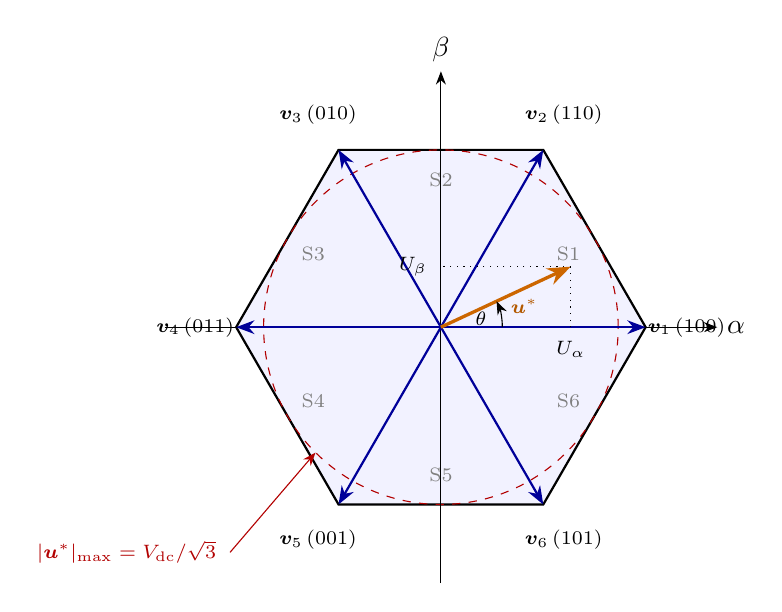
\begin{tikzpicture}[scale=2.6,>=Stealth]
  \def\R{1.0}
  % hexagon
  \draw[thick,fill=blue!5]
    (0:\R) -- (60:\R) -- (120:\R) -- (180:\R) -- (240:\R) -- (300:\R) -- cycle;
  % inscribed circle
  \draw[dashed,red!70!black] (0,0) circle ({\R*0.8660});
  % axes
  \draw[->] (-1.35,0) -- (1.35,0) node[right] {$\alpha$};
  \draw[->] (0,-1.25) -- (0,1.25) node[above] {$\beta$};
  % active vectors
  \foreach \k/\lab/\sw in {0/1/100,60/2/110,120/3/010,180/4/011,240/5/001,300/6/101}{
    \draw[->,thick,blue!60!black] (0,0) -- (\k:\R);
    \node[font=\scriptsize] at (\k:{\R+0.20}) {$\bm{v}_{\lab}\,(\sw)$};
  }
  % reference
  \draw[->,very thick,orange!80!black] (0,0) -- (25:0.70);
  \node[font=\scriptsize,orange!70!black] at (14:0.42) {$\bm{u}^{*}$};
  \draw[dotted] (25:0.70) -- ({0.70*cos(25)},0);
  \node[font=\scriptsize,below] at ({0.70*cos(25)},-0.02) {$U_\alpha$};
  \draw[dotted] (25:0.70) -- (0,{0.70*sin(25)});
  \node[font=\scriptsize,left] at (-0.02,{0.70*sin(25)}) {$U_\beta$};
  \draw[->] (0.30,0) arc (0:25:0.30);
  \node[font=\scriptsize] at (12:0.20) {$\theta$};
  % sector labels
  \node[font=\scriptsize,gray] at (30:0.72) {S1};
  \node[font=\scriptsize,gray] at (90:0.72) {S2};
  \node[font=\scriptsize,gray] at (150:0.72) {S3};
  \node[font=\scriptsize,gray] at (210:0.72) {S4};
  \node[font=\scriptsize,gray] at (270:0.72) {S5};
  \node[font=\scriptsize,gray] at (330:0.72) {S6};
  \node[font=\scriptsize,red!70!black,anchor=east] at (-1.05,-1.10)
        {$|\bm{u}^*|_{\max}=\vdc/\sqrt{3}$};
  \draw[red!70!black,-{Stealth}] (-1.03,-1.10) -- (225:0.866);
\end{tikzpicture}
\caption{Hexagon of the two-level inverter, sector numbering and the inscribed
circle bounding the linear modulation range. Active vector length is
$\tfrac{2}{3}\vdc$.}
\label{fig:hex}
\end{figure}

\subsection{Modulation index}

Two definitions are common. Referred to the linear limit:
\begin{equation}
m = \frac{|\vs|}{\vdc/\sqrt{3}} = \frac{\sqrt{3}\,|\vs|}{\vdc} \in [0,1].
\end{equation}
Referred to the half DC link (the classical PWM definition):
\begin{equation}
M = \frac{\hat{U}_{\text{ph}}}{\vdc/2}, \qquad M_{\max} = \frac{2}{\sqrt{3}} \approx 1.1547 .
\end{equation}
Sinusoidal PWM without injection is limited to $\hat U_{\text{ph}} = \vdc/2$, so both
SVM and third-harmonic injection provide a $15.47\,\%$ increase of the available
fundamental voltage for the same DC link.

\section{Classical space vector modulation}

\subsection{Principle}

Over one switching period $\Ts$ the reference is synthesised as the volt-second
average of the two active vectors adjacent to it, $\bm{v}_k$ and $\bm{v}_{k+1}$,
plus the zero vectors:
\begin{equation}
\vs\,\Ts = \bm{v}_k\,t_k + \bm{v}_{k+1}\,t_{k+1}, \qquad
t_0 = \Ts - t_k - t_{k+1} \ge 0 .
\label{eq:voltsec}
\end{equation}

\subsection{Sector identification}

Two equivalent methods are used.

\paragraph{Angle method.} Compute $\theta = \operatorname{atan2}(\ubeta,\ualpha)$,
wrap to $[0,2\pi)$, then $k = \lfloor \theta/(\pi/3) \rfloor + 1$. Simple but
requires an arctangent.

\paragraph{Sign method (preferred in firmware).} Build the three projections of the
reference on the phase axes, from the inverse Clarke transformation \eqref{eq:clarke}:
\begin{equation}
u_a = \ualpha, \qquad
u_b = -\frac{1}{2}\ualpha + \frac{\sqrt{3}}{2}\ubeta, \qquad
u_c = -\frac{1}{2}\ualpha - \frac{\sqrt{3}}{2}\ubeta .
\label{eq:invclarke}
\end{equation}
The sector boundaries at multiples of $60^\circ$ coincide exactly with the sign
changes of the \emph{differences} $u_a - u_b$, $u_b - u_c$, $u_c - u_a$, since
\begin{equation}
u_b - u_c = \sqrt{3}\,\ubeta, \qquad
u_a - u_b = \frac{3}{2}\ualpha - \frac{\sqrt{3}}{2}\ubeta, \qquad
u_c - u_a = -\frac{3}{2}\ualpha - \frac{\sqrt{3}}{2}\ubeta ,
\end{equation}
which vanish respectively at $\theta = 0^\circ,180^\circ$; $60^\circ,240^\circ$;
$120^\circ,300^\circ$. Equivalently, \emph{the sector is determined by the ordering of
$u_a$, $u_b$, $u_c$}. Forming the binary word
\begin{equation}
N = 1\cdot[u_a > u_b] + 2\cdot[u_b > u_c] + 4\cdot[u_c > u_a]
\end{equation}
gives the look-up of Table~\ref{tab:sector}: three additions and three comparisons,
no trigonometry.

\begin{table}[h]
\centering
\footnotesize
\setlength{\tabcolsep}{4pt}
\begin{tabular}{lcccccc}
\toprule
Ordering & $u_a>u_b>u_c$ & $u_b>u_a>u_c$ & $u_b>u_c>u_a$ & $u_c>u_b>u_a$ & $u_c>u_a>u_b$ & $u_a>u_c>u_b$ \\
$N$ & 3 & 2 & 6 & 4 & 5 & 1 \\
Sector $k$ & 1 & 2 & 3 & 4 & 5 & 6 \\
\bottomrule
\end{tabular}
\caption{Sector look-up from the ordering of the phase projections. Note that the
same $\max$/$\min$ information is what the min--max scheme of
Section~\ref{sec:minmax} uses directly.}
\label{tab:sector}
\end{table}

\subsection{On-times: closed form}

Projecting \eqref{eq:voltsec} on the real and imaginary axes and solving the
$2\times 2$ system gives, for a generic sector $k$,
\begin{align}
t_k       &= \frac{\sqrt{3}\,\Ts}{\vdc}
             \left[\, \ualpha \sin\!\left(\frac{k\pi}{3}\right)
                     - \ubeta \cos\!\left(\frac{k\pi}{3}\right) \right], \label{eq:tk}\\[2mm]
t_{k+1}   &= \frac{\sqrt{3}\,\Ts}{\vdc}
             \left[\, -\ualpha \sin\!\left(\frac{(k-1)\pi}{3}\right)
                     + \ubeta \cos\!\left(\frac{(k-1)\pi}{3}\right) \right], \label{eq:tk1}\\[2mm]
t_0       &= \Ts - t_k - t_{k+1}.
\end{align}

\paragraph{Example: sector 1.} With $k=1$, $\bm{v}_1 = \tfrac{2}{3}\vdc$ and
$\bm{v}_2 = \tfrac{2}{3}\vdc e^{j\pi/3}$, \eqref{eq:voltsec} reads
\begin{align}
\ualpha \Ts &= \frac{2}{3}\vdc\left(t_1 + \frac{1}{2} t_2\right), \\
\ubeta  \Ts &= \frac{2}{3}\vdc\left(\frac{\sqrt{3}}{2} t_2\right),
\end{align}
hence
\begin{equation}
t_1 = \frac{\Ts}{\vdc}\left(\frac{3}{2}\ualpha - \frac{\sqrt{3}}{2}\ubeta\right),
\qquad
t_2 = \frac{\sqrt{3}\,\Ts}{\vdc}\,\ubeta ,
\end{equation}
in agreement with \eqref{eq:tk}--\eqref{eq:tk1}.

\subsection{Auxiliary-variable formulation}

For fixed-point implementations it is convenient to precompute three quantities
independent of the sector:
\begin{equation}
X = \frac{\sqrt{3}\,\Ts}{\vdc}\,\ubeta, \qquad
Y = \frac{\Ts}{\vdc}\left(\frac{3}{2}\ualpha + \frac{\sqrt{3}}{2}\ubeta\right), \qquad
Z = \frac{\Ts}{\vdc}\left(-\frac{3}{2}\ualpha + \frac{\sqrt{3}}{2}\ubeta\right),
\end{equation}
from which the on-times follow by a simple table (Table~\ref{tab:xyz}).

\begin{table}[h]
\centering
\begin{tabular}{lcccccc}
\toprule
Sector $k$ & 1 & 2 & 3 & 4 & 5 & 6 \\
\midrule
$t_k$      & $-Z$ & $Y$  & $X$  & $Z$  & $-Y$ & $-X$ \\
$t_{k+1}$  & $X$  & $Z$  & $-Y$ & $-X$ & $-Z$ & $Y$ \\
\bottomrule
\end{tabular}
\caption{On-times of the two adjacent active vectors from $X$, $Y$, $Z$.}
\label{tab:xyz}
\end{table}

\subsection{Zero-vector split and switching sequence}

The zero interval $t_0$ is distributed between $\bm{v}_0$ (000) and $\bm{v}_7$ (111)
according to a factor $k_0 \in [0,1]$:
\begin{equation}
t_{000} = k_0\,t_0, \qquad t_{111} = (1-k_0)\,t_0 .
\end{equation}
The choice $k_0 = 0.5$ gives \emph{symmetric} (centre-aligned) SVM, which minimises
the current ripple and produces the well-known double-edge pattern. Other choices
generate the discontinuous PWM family: $k_0 = 1$ or $k_0 = 0$ give DPWMMIN and
DPWMMAX, alternating values give DPWM0--DPWM3, each clamping one phase for $120^\circ$
and reducing switching losses by up to one third.

For sector 1 the symmetric sequence over one period is
\begin{equation}
000 \rightarrow 100 \rightarrow 110 \rightarrow 111 \rightarrow 110 \rightarrow 100 \rightarrow 000,
\end{equation}
i.e.\ only one leg commutates at each transition.

\begin{figure}[h]
\centering
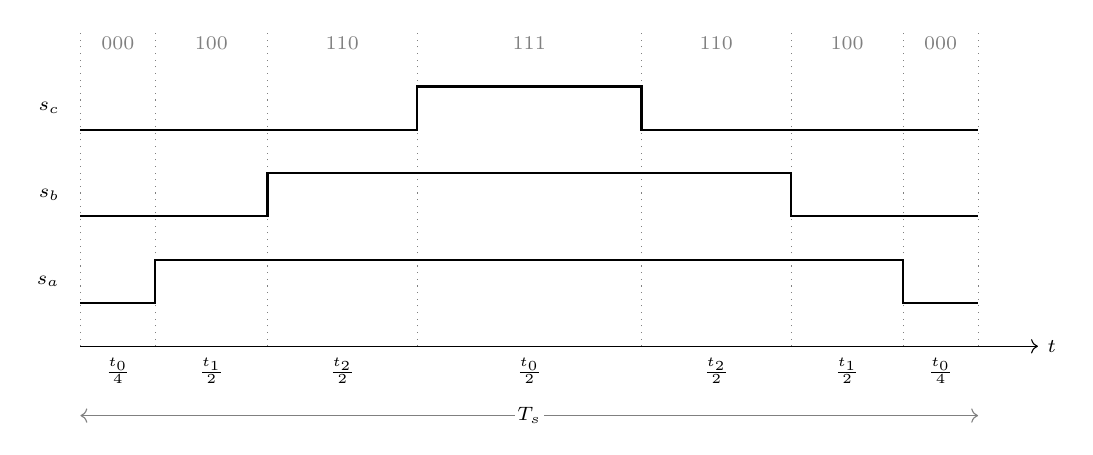
\begin{tikzpicture}[xscale=0.95,yscale=0.55]
  % interval boundaries: 0 | 1 | 2.5 | 4.5 | 7.5 | 9.5 | 11 | 12
  \foreach \x in {0,1,2.5,4.5,7.5,9.5,11,12}{\draw[dotted,gray] (\x,-1.0) -- (\x,6.3);}
  % state labels on top
  \foreach \x/\lab in {0.5/000,1.75/100,3.5/110,6.0/111,8.5/110,10.25/100,11.5/000}{
     \node[font=\scriptsize,gray] at (\x,6.0) {\lab};}
  % s_c (top trace)
  \draw[thick] (0,4) -- (4.5,4) -- (4.5,5) -- (7.5,5) -- (7.5,4) -- (12,4);
  \node[left,font=\scriptsize] at (-0.15,4.5) {$s_c$};
  % s_b
  \draw[thick] (0,2) -- (2.5,2) -- (2.5,3) -- (9.5,3) -- (9.5,2) -- (12,2);
  \node[left,font=\scriptsize] at (-0.15,2.5) {$s_b$};
  % s_a
  \draw[thick] (0,0) -- (1,0) -- (1,1) -- (11,1) -- (11,0) -- (12,0);
  \node[left,font=\scriptsize] at (-0.15,0.5) {$s_a$};
  % time axis
  \draw[->] (0,-1.0) -- (12.8,-1.0) node[right,font=\scriptsize] {$t$};
  \foreach \x/\lab in {0.5/{\frac{t_0}{4}},1.75/{\frac{t_1}{2}},3.5/{\frac{t_2}{2}},
                       6.0/{\frac{t_0}{2}},8.5/{\frac{t_2}{2}},10.25/{\frac{t_1}{2}},
                       11.5/{\frac{t_0}{4}}}{
     \node[font=\scriptsize,below] at (\x,-1.05) {$\lab$};}
  \draw[<->,gray] (0,-2.6) -- (12,-2.6);
  \node[font=\scriptsize,fill=white,inner sep=1pt] at (6,-2.6) {$\Ts$};
\end{tikzpicture}
\caption{Symmetric (centre-aligned) switching pattern in sector 1 over one period.
Only one leg commutates at each state transition; the zero time is split equally
between $\bm{v}_0$ at the edges and $\bm{v}_7$ in the middle.}
\end{figure}

\subsection{From on-times to duty cycles}

Counting, for each leg, the total time during which its upper device is on gives the
duty cycles collected in Table~\ref{tab:duty}. All entries are divided by $\Ts$.

\begin{table}[h]
\centering
\renewcommand{\arraystretch}{1.35}
\begin{tabular}{cccc}
\toprule
Sector & $d_a$ & $d_b$ & $d_c$ \\
\midrule
1 & $(t_1+t_2+\tfrac{t_0}{2})/\Ts$ & $(t_2+\tfrac{t_0}{2})/\Ts$ & $\tfrac{t_0}{2\Ts}$ \\
2 & $(t_2+\tfrac{t_0}{2})/\Ts$ & $(t_2+t_3+\tfrac{t_0}{2})/\Ts$ & $\tfrac{t_0}{2\Ts}$ \\
3 & $\tfrac{t_0}{2\Ts}$ & $(t_3+t_4+\tfrac{t_0}{2})/\Ts$ & $(t_4+\tfrac{t_0}{2})/\Ts$ \\
4 & $\tfrac{t_0}{2\Ts}$ & $(t_4+\tfrac{t_0}{2})/\Ts$ & $(t_4+t_5+\tfrac{t_0}{2})/\Ts$ \\
5 & $(t_6+\tfrac{t_0}{2})/\Ts$ & $\tfrac{t_0}{2\Ts}$ & $(t_5+t_6+\tfrac{t_0}{2})/\Ts$ \\
6 & $(t_6+t_1+\tfrac{t_0}{2})/\Ts$ & $\tfrac{t_0}{2\Ts}$ & $(t_6+\tfrac{t_0}{2})/\Ts$ \\
\bottomrule
\end{tabular}
\caption{Duty cycles of the three legs for symmetric SVM ($k_0 = 0.5$).
$t_k$ and $t_{k+1}$ are the on-times of the two active vectors of the sector.}
\label{tab:duty}
\end{table}

The duty cycles are then written to the compare registers of a centre-aligned
(up--down counting) timer, so that the resulting pattern is automatically symmetric
about the middle of the period.

\section{Triangular third-harmonic injection (min--max)}
\label{sec:minmax}

\subsection{Zero-sequence degree of freedom}

For an isolated-neutral load, the line-to-line voltages -- and therefore the currents
-- depend only on the \emph{differences} between the leg references. Adding the same
signal $u_0$ to all three phase references leaves the load voltages unchanged:
\begin{equation}
u_x' = u_x + u_0, \qquad x \in \{a,b,c\} \quad\Longrightarrow\quad
u_{xy}' = u_{xy}.
\end{equation}
This zero-sequence component is a free design variable, and it can be used to keep
the modulating signals within the linear range for a larger fundamental amplitude.

\subsection{The min--max (triangular) choice}

Starting from $(\ualpha, \ubeta)$, compute the phase references with the inverse
Clarke transformation:
\begin{equation}
u_a = \ualpha, \qquad
u_b = -\frac{1}{2}\ualpha + \frac{\sqrt{3}}{2}\ubeta, \qquad
u_c = -\frac{1}{2}\ualpha - \frac{\sqrt{3}}{2}\ubeta .
\end{equation}
Then choose the zero-sequence that centres the three references about zero:
\begin{equation}
\boxed{\;
u_0 = -\frac{\max(u_a,u_b,u_c) + \min(u_a,u_b,u_c)}{2}
\;}
\label{eq:minmax}
\end{equation}
and obtain the duty cycles directly:
\begin{equation}
\boxed{\;
d_x = \frac{1}{2} + \frac{u_x + u_0}{\vdc}, \qquad x \in \{a,b,c\}.
\;}
\label{eq:duty}
\end{equation}
No sector identification, no trigonometry, no look-up table: three additions, one
sorting network of three elements, and three multiply-adds.

\subsection{Properties of the injected waveform}

For a balanced sinusoidal reference of peak $\hat U$ and angle $\theta = \omega t$,
\eqref{eq:minmax} produces a \emph{triangular} waveform of period $120^\circ$, i.e.\
at three times the fundamental frequency, with peak value
\begin{equation}
\hat{u}_0 = \frac{\hat U}{4}.
\end{equation}
Sampling a few points illustrates the shape: at $\theta=0^\circ$,
$u_0 = -\hat U/4$; at $\theta = 30^\circ$, $u_0 = 0$; at $\theta = 60^\circ$,
$u_0 = +\hat U/4$.

Its Fourier expansion contains only odd triplen harmonics:
\begin{equation}
u_0(\theta) = -\frac{2\hat U}{\pi^2}
\sum_{n = 1,3,5,\dots} \frac{\cos(3n\theta)}{n^2}
= -\,0.2026\,\hat U \cos 3\theta - 0.0225\,\hat U \cos 9\theta - \dots
\end{equation}
All of these are zero-sequence components: with an isolated neutral they cannot
drive current and do not appear in the load voltages.

\begin{figure}[h]
\centering
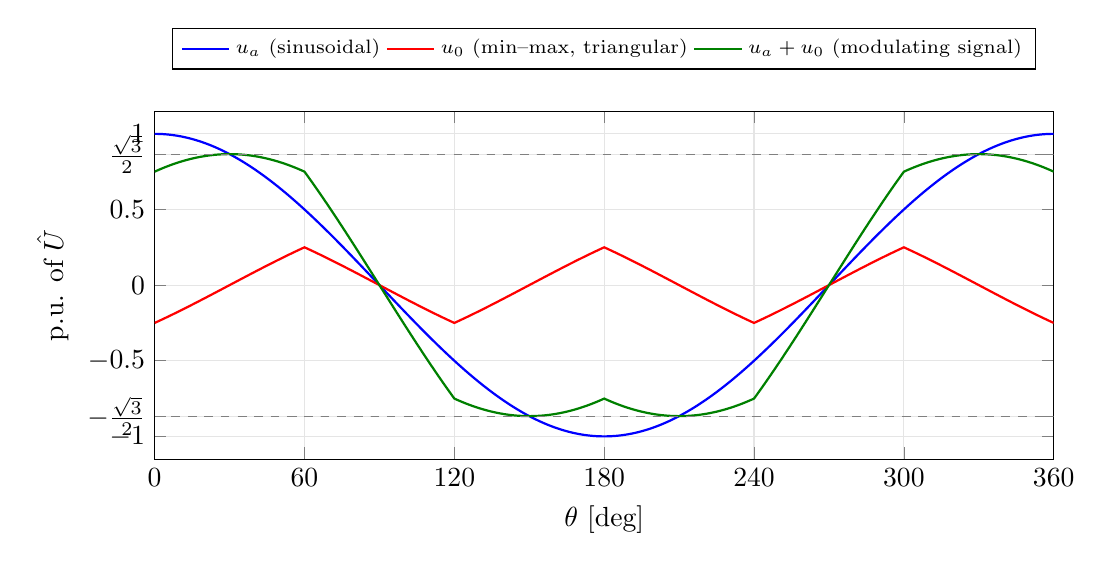
\begin{tikzpicture}
\begin{axis}[
  width=13cm, height=6cm,
  xlabel={$\theta$ [deg]}, ylabel={p.u. of $\hat U$},
  xmin=0, xmax=360, ymin=-1.15, ymax=1.15,
  xtick={0,60,...,360},
  ytick={-1,-0.866,-0.5,0,0.5,0.866,1},
  yticklabels={$-1$,$-\frac{\sqrt3}{2}$,$-0.5$,$0$,$0.5$,$\frac{\sqrt3}{2}$,$1$},
  grid=both, grid style={gray!20},
  legend style={font=\scriptsize, at={(0.5,1.24)}, anchor=north, legend columns=3},
  samples=721, domain=0:360
]
\addplot[blue,thick] {cos(x)};
\addlegendentry{$u_a$ (sinusoidal)}
\addplot[red,thick] {-0.5*(max(max(cos(x),cos(x-120)),cos(x+120)) + min(min(cos(x),cos(x-120)),cos(x+120)))};
\addlegendentry{$u_0$ (min--max, triangular)}
\addplot[green!50!black,thick] {cos(x) - 0.5*(max(max(cos(x),cos(x-120)),cos(x+120)) + min(min(cos(x),cos(x-120)),cos(x+120)))};
\addlegendentry{$u_a + u_0$ (modulating signal)}
\addplot[dashed,gray] {0.866};
\addplot[dashed,gray] {-0.866};
\end{axis}
\end{tikzpicture}
\caption{Sinusoidal reference of unit peak, triangular zero-sequence produced by the
min--max rule, and the resulting modulating signal. The peak of the modulating signal
is $\sqrt{3}/2 \approx 0.866$ instead of $1$, which is exactly the $15.47\,\%$
headroom gained.}
\label{fig:inj}
\end{figure}

\subsection{Why the range extends}

The modulating signal $u_a + u_0$ has a peak of $\tfrac{\sqrt{3}}{2}\hat U$, reached
at $\theta = 30^\circ$ (Fig.~\ref{fig:inj}). Linear operation requires
$\left| u_x + u_0 \right| \le \vdc/2$, hence
\begin{equation}
\frac{\sqrt{3}}{2}\hat U \le \frac{\vdc}{2}
\quad\Longrightarrow\quad
\hat U \le \frac{\vdc}{\sqrt{3}},
\end{equation}
which is exactly the limit \eqref{eq:limit} obtained from the hexagon geometry.

\subsection{Comparison with sinusoidal third-harmonic injection}

A related scheme injects a pure sinusoid,
\begin{equation}
u_0 = -\frac{\hat U}{6}\cos 3\theta ,
\end{equation}
whose $1/6$ coefficient minimises the peak of the resulting modulating signal. This
also reaches $\tfrac{\sqrt{3}}{2}\hat U$ and therefore the same voltage limit, but it
requires knowledge of the reference angle and amplitude and it is \emph{not} exactly
equivalent to SVM: the instantaneous ripple and the switching pattern differ slightly.
The triangular (min--max) form is preferred because it needs no angle information,
works instantaneously on any reference (including transients and unbalanced or
non-sinusoidal references) and coincides exactly with symmetric SVM.

\section{Equivalence of the two methods}

\begin{quote}
\emph{Symmetric SVM with $k_0 = 0.5$ and carrier-based modulation with min--max
injection produce identical duty cycles.}
\end{quote}

\paragraph{Proof for sector 1.} In sector $1$ ($0 \le \theta < 60^\circ$) one has
$u_a > u_b > u_c$, so $\max = u_a$, $\min = u_c$ and
\begin{equation}
u_0 = -\frac{u_a + u_c}{2}
    = -\frac{1}{2}\left(\ualpha - \frac{1}{2}\ualpha - \frac{\sqrt{3}}{2}\ubeta\right)
    = -\frac{\ualpha}{4} + \frac{\sqrt{3}}{4}\ubeta .
\end{equation}
Equation \eqref{eq:duty} then gives
\begin{equation}
d_a = \frac{1}{2} + \frac{1}{\vdc}\left(\frac{3}{4}\ualpha + \frac{\sqrt{3}}{4}\ubeta\right).
\label{eq:da_inj}
\end{equation}
From the SVM side, with
$t_1/\Ts = \left(\tfrac{3}{2}\ualpha - \tfrac{\sqrt{3}}{2}\ubeta\right)/\vdc$,
$t_2/\Ts = \sqrt{3}\,\ubeta/\vdc$ and
$t_0/\Ts = 1 - \left(\tfrac{3}{2}\ualpha + \tfrac{\sqrt{3}}{2}\ubeta\right)/\vdc$,
Table~\ref{tab:duty} gives
\begin{align}
d_a &= \frac{t_1 + t_2}{\Ts} + \frac{t_0}{2\Ts}
     = \frac{1}{\vdc}\left(\frac{3}{2}\ualpha + \frac{\sqrt{3}}{2}\ubeta\right)
       + \frac{1}{2} - \frac{1}{2\vdc}\left(\frac{3}{2}\ualpha + \frac{\sqrt{3}}{2}\ubeta\right) \nonumber\\
    &= \frac{1}{2} + \frac{1}{\vdc}\left(\frac{3}{4}\ualpha + \frac{\sqrt{3}}{4}\ubeta\right),
\end{align}
which coincides with \eqref{eq:da_inj}. The same holds for $d_b$, $d_c$ and, by the
$60^\circ$ symmetry of the problem, for all sectors. $\blacksquare$

\paragraph{Consequence.} There is no performance argument for the sector-based
implementation. The min--max form is preferred in practice; the geometric SVM
description remains the natural language for reasoning about vector selection,
overmodulation and multilevel extensions.

\section{Implementation}

\subsection{Classical SVM}

\begin{lstlisting}[caption={Sector-based SVM.}]
void svm_classic(float ua, float ub, float vdc, float *da, float *db, float *dc)
{
    /* phase projections (inverse Clarke) */
    const float va =  ua;
    const float vb = -0.5f*ua + 0.8660254f*ub;
    const float vc = -0.5f*ua - 0.8660254f*ub;

    /* sector from the ordering of the projections */
    int N = (va > vb) + 2*(vb > vc) + 4*(vc > va);
    static const int sect_lut[8] = {0, 6, 2, 1, 4, 5, 3, 0};
    int k = sect_lut[N];                    /* 1..6 */

    /* auxiliary variables, normalised to Ts */
    const float X =  1.7320508f*ub / vdc;
    const float Y = ( 1.5f*ua + 0.8660254f*ub) / vdc;
    const float Z = (-1.5f*ua + 0.8660254f*ub) / vdc;

    float t1, t2;
    switch (k) {
        case 1: t1 = -Z; t2 =  X; break;
        case 2: t1 =  Y; t2 =  Z; break;
        case 3: t1 =  X; t2 = -Y; break;
        case 4: t1 =  Z; t2 = -X; break;
        case 5: t1 = -Y; t2 = -Z; break;
        default:t1 = -X; t2 =  Y; break;
    }

    /* overmodulation: scale back onto the hexagon boundary */
    float sum = t1 + t2;
    if (sum > 1.0f) { t1 /= sum; t2 /= sum; sum = 1.0f; }

    const float t0h = 0.5f*(1.0f - sum);    /* t0/(2*Ts) */

    switch (k) {
        case 1: *da = t1+t2+t0h; *db = t2+t0h;    *dc = t0h;       break;
        case 2: *da = t1+t0h;    *db = t1+t2+t0h; *dc = t0h;       break;
        case 3: *da = t0h;       *db = t1+t2+t0h; *dc = t2+t0h;    break;
        case 4: *da = t0h;       *db = t1+t0h;    *dc = t1+t2+t0h; break;
        case 5: *da = t2+t0h;    *db = t0h;       *dc = t1+t2+t0h; break;
        default:*da = t1+t2+t0h; *db = t0h;       *dc = t1+t0h;    break;
    }
}
\end{lstlisting}

\noindent
Note that in the second switch the on-time associated with the \emph{first} vector of
the sector, $t_1$, and that of the \emph{second}, $t_2$, swap roles between odd and
even sectors, consistently with Table~\ref{tab:duty}.

\subsection{Min--max injection}

\begin{lstlisting}[caption={Carrier-based SVM with triangular injection.}]
void svm_minmax(float ua, float ub, float vdc, float *da, float *db, float *dc)
{
    /* inverse Clarke */
    float va =  ua;
    float vb = -0.5f*ua + 0.8660254f*ub;
    float vc = -0.5f*ua - 0.8660254f*ub;

    /* min and max of the three references */
    float vmax = va > vb ? (va > vc ? va : vc) : (vb > vc ? vb : vc);
    float vmin = va < vb ? (va < vc ? va : vc) : (vb < vc ? vb : vc);

    /* triangular zero sequence */
    float v0 = -0.5f*(vmax + vmin);

    const float inv = 1.0f / vdc;
    *da = 0.5f + (va + v0)*inv;
    *db = 0.5f + (vb + v0)*inv;
    *dc = 0.5f + (vc + v0)*inv;

    /* saturation (enters overmodulation) */
    *da = *da < 0.0f ? 0.0f : (*da > 1.0f ? 1.0f : *da);
    *db = *db < 0.0f ? 0.0f : (*db > 1.0f ? 1.0f : *db);
    *dc = *dc < 0.0f ? 0.0f : (*dc > 1.0f ? 1.0f : *dc);
}
\end{lstlisting}

\section{Practical notes}

\begin{itemize}
\item \textbf{Timer configuration.} Use a centre-aligned (up--down) counter with
period $N$ and load $\mathrm{CCR}_x = (1-d_x)\,N$ or $d_x N$ depending on the output
polarity. Update the compare registers through the preload registers, synchronised
with the counter underflow, to avoid glitches.

\item \textbf{Sampling.} Sample the currents at the counter underflow (and, for
double-update schemes, also at overflow): at those instants a zero vector is applied
and the sampled value is the average of the ripple.

\item \textbf{Dead time.} Dead time introduces a volt-second error whose sign depends
on the current polarity, producing $5^\text{th}$ and $7^\text{th}$ harmonics and
distortion around the current zero crossings. Compensate either in the duty cycles or
in the voltage reference.

\item \textbf{Minimum pulse width.} Pulses shorter than the device transition time
plus the dead time cannot be reproduced. Either suppress them (pulse dropping) or
merge them, and account for the resulting voltage error.

\item \textbf{DC-link feedforward.} Use the measured $\vdc$ in \eqref{eq:duty} so
that DC-link ripple does not propagate into the output voltage.

\item \textbf{Overmodulation.} Beyond $|\vs| = \vdc/\sqrt{3}$ the reference leaves
the inscribed circle. Simple saturation of the duty cycles gives a smooth but
nonlinear transfer characteristic; dedicated mode-I / mode-II algorithms preserve the
fundamental gain up to six-step operation ($\hat U = \tfrac{2}{\pi}\vdc$), at the cost
of low-order harmonics. Anti-windup on the current controllers is mandatory in this
region.

\item \textbf{Discontinuous PWM.} Replacing \eqref{eq:minmax} with
$u_0 = \tfrac{\vdc}{2}\operatorname{sgn}(u_{\max}) - u_{\max}$ (or the analogous
expression with $u_{\min}$) clamps one leg at a time, reducing switching losses.
The clamping window can be aligned with the current peak to maximise the benefit,
which is useful at high modulation index.
\end{itemize}

\section{Summary}

\begin{table}[h]
\centering
\begin{tabular}{p{4.6cm}p{4.6cm}p{4.6cm}}
\toprule
& \textbf{Classical SVM} & \textbf{Min--max injection} \\
\midrule
Sector detection & required & not required \\
Trigonometry & optional (sign method avoids it) & none \\
Operations per period & $\sim$20 plus branches & $\sim$12, branch-light \\
Zero-vector split & explicit ($k_0$) & implicit ($k_0 = 0.5$) \\
Linear limit $\hat U_{\text{ph}}$ & $\vdc/\sqrt{3}$ & $\vdc/\sqrt{3}$ \\
Output waveform & \multicolumn{2}{c}{identical for $k_0 = 0.5$} \\
Best suited to & vector reasoning, DPWM variants, multilevel & production firmware \\
\bottomrule
\end{tabular}
\caption{Comparison of the two implementations.}
\end{table}

Both methods start from the same pair $(\ualpha, \ubeta)$ and end with three duty
cycles in $[0,1]$. The classical formulation makes the geometry explicit and is the
right framework for overmodulation and multilevel topologies; the min--max
formulation is the compact and numerically robust way of implementing it.

\end{document}
